\documentclass[gchron, manuscript]{copernicus}

\usepackage{hyperref,caption}

\begin{document}

\title{FAIR fission track analysis with geochron@home}

\Author[1][p.vermeesch@ucl.ac.uk]{Pieter}{Vermeesch}
\Author[1]{Tim}{Band}
\Author[2]{Jiangping}{He}
\Author[1]{Rex}{Galbraith}
\Author[3]{Andrew}{Carter}

\affil[1]{University College London, London WC1E 6BT, United Kingdom}
\affil[2]{King's College London, London SE1 8WA, United Kingdom}
\affil[3]{Birkbeck, University of London, London WC1E 7HX, United Kingdom}

\runningtitle{FAIR fission track analysis with geochron@home}

\runningauthor{P Vermeesch \emph{et al.}}

\received{}
\pubdiscuss{} %% only important for two-stage journals
\revised{}
\accepted{}
\published{}

\firstpage{1}

\maketitle

\begin{abstract}
Fission track thermochronology is based on the visual analysis of
optical images. This visual process is prone to observer bias. Fission
track datasets are currently reported as small data tables. The
interpretation of these tables requires a high degree of trust between
the fission track analyst and the user of the data. geochron@home is
software that removes this requirement of trust. It combines a
browser-based `virtual microscope' with an online database to provide
FAIR (Findable, Accessible, Interoperable and Reproducible) access to
fission track data.\medskip

geochron@home serves four different purposes. It can be used (1) to
count fission tracks in `private mode', i.e. hidden from other users
on the internet; (2) to archive fission track images and counts for
inspection by other users; (3) to create tutorials for new students of
the fission track method; and (4) to serve randomly selected
selections of images to citizen scientists. We illustrate these four
applications with examples that demonstrate (1) geochron@home's
ability to compare and combine fission track counts for multiple users
within a lab group; (2) the value of the geochron@home archive in the
peer review system; (3) the use of simple tutorials in teaching novice
users how to count fission tracks; and (4) the opportunities and
challenges of crowd-sourced fission track analysis.\medskip

geochron@home was written in Python and Javascript. Its code is freely
available for inspection and modification, allowing users to set up
their own geochron@home server. Alternatively, users who would like to
upload data to the archive, but do not have the facilities to set up
their own server, may use the server at University College London free
of charge. The archive accepts image stacks acquired on any type of
digital microscope, and accomodates fission track data (counts and
length measurements) from external fission track analysis suites such
as Fission Track Studio and Track\emph{Flow}.\medskip

We anticipate that the introduction of FAIR workflows will make
fission track data more accurate and more future proof. Storing
fission track data online will benefit future developments in fission
track thermochronology. For example, archival datasets of peer
reviewed fission track counts can be used to train and improve machine
learning algorithms for automated fission track analysis. We invite
other geochronological methods to follow the fission track community's
lead in FAIR data processing. This would benefit all the Earth Science
disciplines that depend on geochronological data.
\end{abstract}

\introduction\label{sec:intro}

Science is on an irreversible trajectory towards greater
openness. Geochronology is no exception to this trend, as this journal
illustrates with its open access and review policies. Funding agencies
increasingly demand that research results and data are shared with the
public. Currently, geochronological data are generally provided as
flat tables of dates or isotopic ratio estimates. However, in other
fields of science such as physics, it is common practice to share the
raw unprocessed measurements along with processing instructions
\citep[e.g.,][]{abbott2016}. This paper moves geochronology in the
same direction. It presents a mechanism to generate and store fully
FAIR \citep[Findable, Accessible, Interoperable and
  Reproducible;][]{wilkinson2016} data in the context of fission track
analysis.\medskip

Unlike most other geochronometers, which require mass spectrometers to
estimate parent-daughter ratios, fission tracks are observed under an
optical microscope and counted by a human observer.  In recent years,
digital microscopy has moved fission track data acquisition from the
ocular lenses of a microscope to the computer screen
\citep{gleadow2009, vanranst2019, gleadow2019}. Ongoing developments
in artificial intelligence generate further opportunities to improve
the throughput and accuracy of fission track data
\citep{nachtergaele2020}. But despite the richness of the digital
datasets produced by these novel tools, fission track data are still
reported as small summary tables. These tables require an unnecessary
degree of trust between the `producer' and `consumer' of the
data.\medskip

geochron@home is a free and open software platform that allows
geochronologists to share their raw fission track data over the
internet for perusal by peer reviewers, colleagues and the general
public. geochron@home is a virtual petrographic microscope connected to a
database with digital image stacks of etched fission track
samples. The platform can be used to acquire, archive and inspect
fission track data in full adherence to the FAIR data principles. In
Section~\ref{sec:architecture}, we will describe geochron@home's software
architecture in five steps. We will show that this architecture
accommodates imagery from any type of digital microscope. It enables
flexible workflows that can be adapted to four different
applications.\medskip

Using image stacks of Mount Dromedary apatite, we will show how
geochron@home can be used to count fission tracks in `private mode'
(Section~\ref{sec:private}); to archive published fission track
datasets in `public mode' (Section~\ref{sec:GaHa}); to build tutorials
for training purposes (Section~\ref{sec:tutorial}); and to
crowd-source fission track data on the internet
(Section~\ref{sec:crowdsourcing}). Because geochron@home is free and
open, it can be extended and improved by any interested party. We make
some suggestions for future improvements in
Section~\ref{sec:outlook}. We hope that the geochron@home's example
will be followed in other geochronological disciplines, as this will
benefit not only geochronology itself, but all the other disciplines
that depend on it (Section~\ref{sec:conclusions}).

\section{Workflow}\label{sec:architecture}

The geochron@home workflow separates the acquisition of microscope
images from their analysis, providing the flexibility to accommodate
data from different microscope manufacturers. The workflow can be
broken down into five steps.

\begin{enumerate}
\item Acquisition of z-stacks of microscope images in reflected and
  transmitted light for each of the grains in a sample and,
  optionally, for the accompanying external detector
  (Figure~\ref{fig:EDM}). At University College London, this first
  step is currently accomplished by a Python macro within Zeiss' Zen
  Blue software.  However, geochron@home can also accommodate imagery
  from other platforms, such as Fission Track Studio
  \citep[Zeiss;][]{gleadow2009} and Track\emph{Flow}
  \citep[Nikon;][]{vanranst2019}.

\item Prepare the z-stacks for uploading to the geochron@home
  database. This database requires that the images are organised as a
  nested sequence of directories, in which a `project' consists of
  `samples' that comprise a number of `grains'.  Each grain
  corresponds to a numbered sequence of \texttt{.jpeg} images, one for
  each layer of the z-stack. Note that the raw microscope images are
  generally not stored as \texttt{.jpeg} files but in uncompressed
  \texttt{.czi} (for Zen Blue), \texttt{.tif} (for Fission Track
  Studio) or \texttt{.nd2} (for Nikon/Track\emph{Flow})
  formats. Conversion from these raw images to sequences of
  \texttt{.jpeg} files is done with a shell script using Imagemagick
  \citep{still2006}.\medskip

  In addition to the sequence of \texttt{.jpeg} images, a low level
  `grain' folder can also include an optional file called
  \texttt{roi.json} containing the vertices of a default region of
  interest for spontaneous (and/or induced) track counting. The
  database structure can also accommodate existing fission track
  counting results.  For example, if a user has already counted their
  fission tracks in Fission Track Studio, then they can store those
  results in a \texttt{.json} file at the `sample' level
  directory. Because Fission Track Studio stores its results in an
  \texttt{.xml} format, a second conversion script was created to
  translate those results into an equivalent \texttt{.json} format.

\item Upload the data to the geochron@home platform. geochron@home is
  a Django web-app with a PostgreSQL database.  The database can be
  accessed via a Python API and a (more limited) web-based
  GUI. Accessing the API requires administrator
  privileges. Administrators can create projects, samples and grains;
  download data; and set the access rights of `ordinary' users.
  Projects can be private or public. The source code and installation
  instructions for geochron@home are freely available over GitHub (see
  the Data Availability statement at the end of this paper). This
  allows fission track users to set up their own
  server. Alternatively, fission track labs can upload their data to
  the UCL server by contacting the corresponding author.

\item Analyse the images with a browser-based `virtual fission track
  microscope' powered by the Leaflet library (JavaScript). This
  virtual instrument acts as a front-end to geochron@home. It has a
  simple user interface with controls to zoom, pan and focus in or out
  of the digital image stack. Depending on the permissions granted to
  the user by the administrator, the virtual microsocope offers a
  number of different options.  Entry level `ordinary' users are only
  allowed to count tracks by clicking within a pre-defined `region of
  interest'. In contrast, `superusers' are allowed to define their own
  regions of interest. Once the user is satisfied that they have
  counted all the fission tracks in a particular grain, they can
  submit the results to the server. They are then presented with a new
  set of images until all grains are counted.

\item Post-processing. The fission track data can either be downloaded
  as a flat data table of counts and areas, or as a \texttt{.json}
  file containing the locations of all the counted
  tracks. geochron@home does not provide any tools to post-process
  these files. They are meant to be passed on to other tools such as
  spreadsheet applications or IsoplotR \citep{vermeesch2018c}.
  
\end{enumerate}
  
The five-step workflow can be used for several applications, including
(1) conventional fission track analysis; (2) archiving published
fission track results; (3) building tutorials; and (4) crowd-sourcing
fission track data. The next sections of this paper will illustrate
these applications with real world examples.\medskip

%\begin{figure}[!ht]
{ \centering 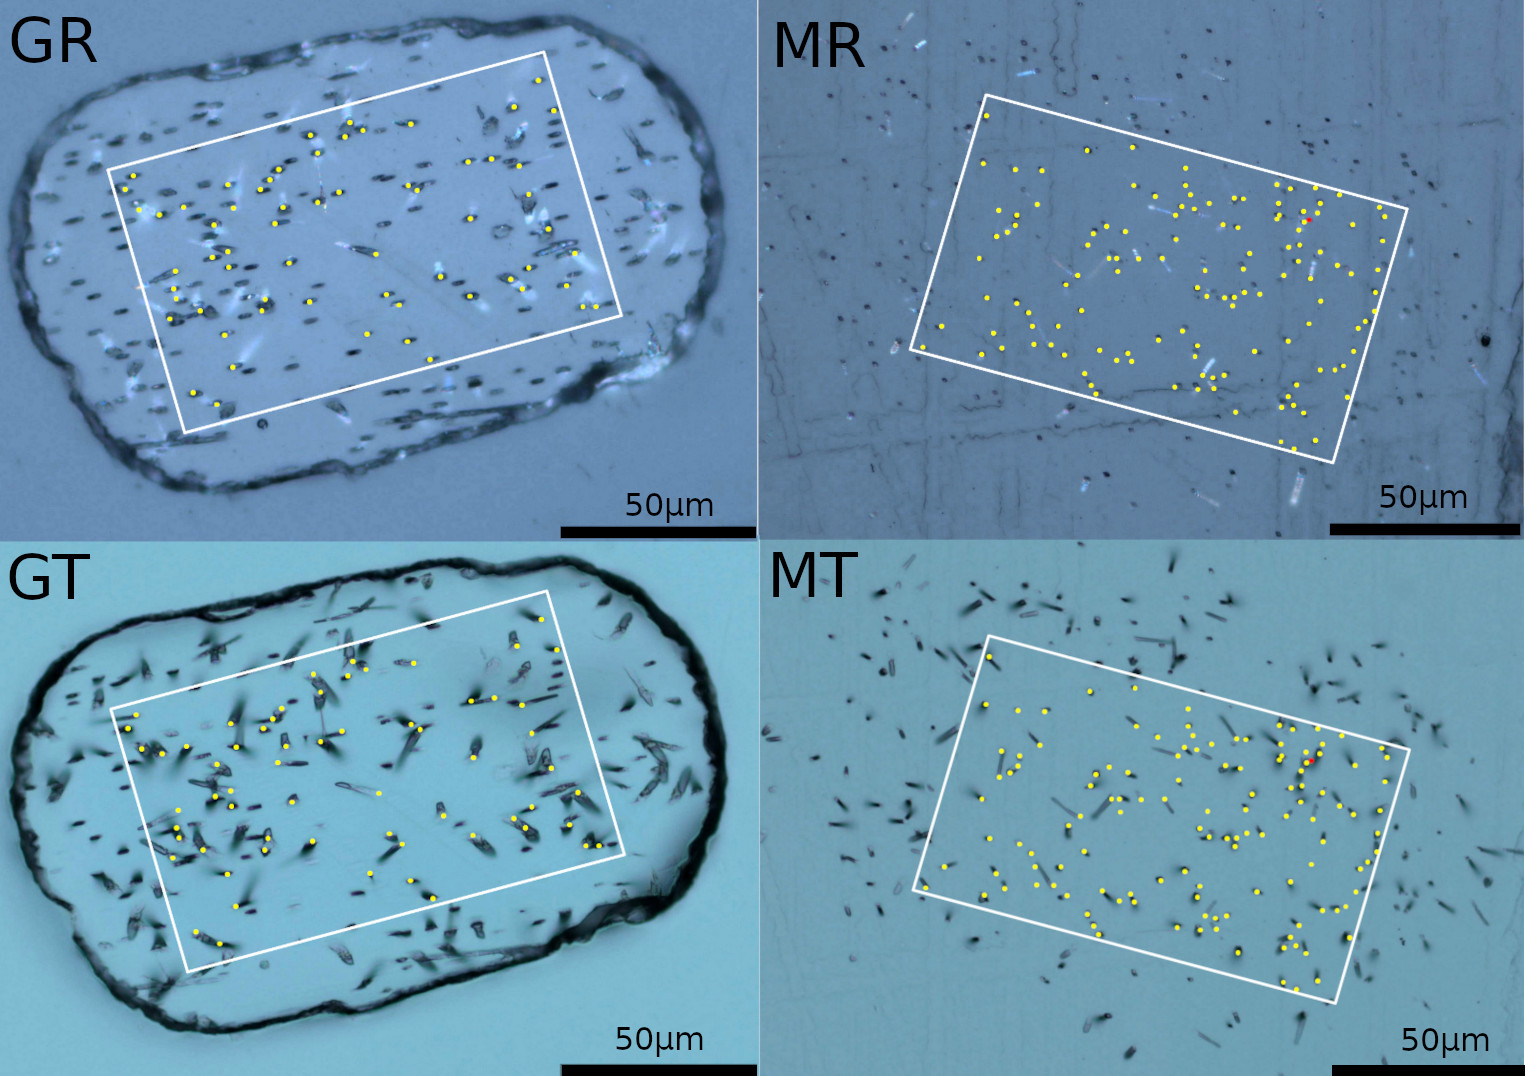
\includegraphics[width=12cm]{EDM.jpg}
  \captionof{figure}{
    Screenshots of raw fission track data for the external detector
    method in geochron@home. GR: an apatite grain in reflected light;
    GT: the same grain in transmitted light; MR: the corresponding
    mica detector in reflected light; MT: the mica detector in
    transmitted light. White rectangles mark the region of interest
    (ROI), within which an analyst has counted fission tracks by
    marking their etch pits (shown in yellow). The raw data for this
    figure can be viewed on the geochron@home archive
    (\url{https://github.com/pvermees/GaHa}).\medskip}
  \label{fig:EDM}
}%\end{figure}

\section{Counting fission tracks in `private mode'}\label{sec:private}

Administrators can define regions of interest (ROI) and count or edit
the fission track coordinates of any grain in a geochron@home
database. They can also assign other users to groups, and give these
groups access to a subset of the projects in the
database. Administrators have fine control over the permissions of the
groups. For example, they can allow the members of one group to define
their own ROIs, whilst requiring members of another group to count
fission tracks in predefined ROIs.  Groups provide a mechanism to
compare and combine the results of multiple analysts of the same
sample. Figure~\ref{fig:AvP} illustrates this with two sets of fission
track density estimates for the same sample of Mount Dromedary apatite
\citep{green1985b}, analysed by two users (PV and AC).\medskip

Let $N_1$ and $N_2$ be the numbers of spontaneous tracks counted by
the two users over areas $A_1$ and $A_2$, respectively. Then their
estimated track densities are given by $\hat{\rho}_1 = N_1/A_1$ and
$\hat{\rho}_2 = N_2/A_2$. In this situation when the two areas
overlap, $N_1$ and $N_2$ cannot be treated as independent Poisson
counts because the two analysts will count some of the same tracks. It
can be shown that, under simple (ideal) assumptions, the uncertainty
of the ratio of the estimated track densities is given approximately
by
\begin{equation}
  \frac{\mbox{se}(\hat{\rho}_1/\hat{\rho}_2)}{\hat{\rho}_1/\hat{\rho}_2} \approx
  \sqrt{ \frac{1}{N_1} + \frac{1}{N_2} - \frac{2\,N_0}{N_1\,N_2} }
  \label{eq:NO}
\end{equation}

\noindent where $N_0$ is the number of tracks counted by both
observers in the area of overlap ($A_0$, say) between their respective
ROIs.\medskip 

The combined data plots of Figures~\ref{fig:AvP}b and c contain two
sets of counts for 25 grains, with $\sum N_{1} = 686$ (PV) and $\sum
N_{2} = 679$ (AC), and a weighted mean track density ratio
$\hat{\rho}_{1}/\hat{\rho}_{1} = 0.94$ with relative standard error
0.013. PV counted 600 tracks in those common areas $A_0$, of which 549
were also counted by AC. Conversely, AC counted 622 tracks of which
549 were also counted by PV. The ratio of the two analysts' track
density estimates based just on the common area is therefore 600/622 =
0.965 with relative standard error 0.018, calculated from
Equation~\ref{eq:NO}, with $N_1 = 686$, $N_2 = 679$ and $N_0 = 549$.
This is close to the weighted mean ratio of 0.94
(Figure~\ref{fig:AvP}c), and is slightly nearer to 1. It indicates
that PV under-counts the Mount Dromedary apatite by 3.5\% relative to
AC.  The existence of `observer bias' is well documented
\citep{tamer2025}.  It is one of the reasons why fission track
analysis is often done relative to age standards: observer bias does
not have to be a problem provided that it is consistent between
grains, and between samples.\medskip

%\begin{figure}[!ht]
{ \centering 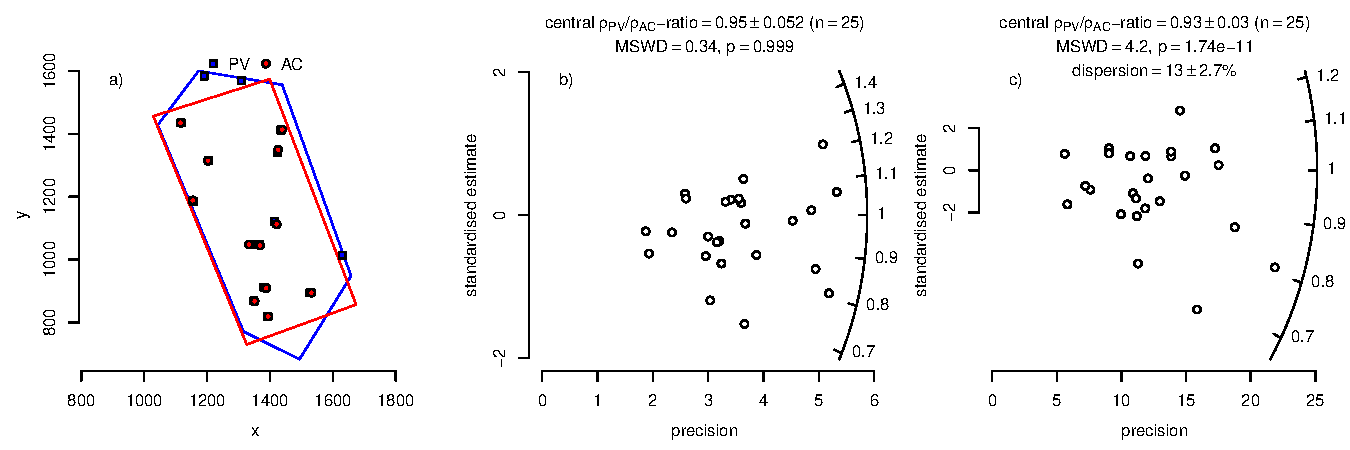
\includegraphics[width=\linewidth]{AvP.pdf}
  \captionof{figure}{Comparison of fission track data for Mount
    Dromedary apatite by two analysts (PV = Pieter Vermeesch and AC =
    Andrew Carter). a) the track counts and ROIs of both users for
    grain~3, shown in blue (PV) and red (AC); b) comparison of the
    track densities for PV and AC for all 25 grains analysed by the
    two analysts with a reference line for
    $\hat{\rho}_\text{PV}=\hat{\rho}_\text{AC}$; c) radial plot of the
    same data, using Equation~\ref{eq:NO}.}
  \label{fig:AvP}
}%\end{figure}

\section{The geochron@home archive (GaHa)}\label{sec:GaHa}

Once a set of fission track images has been analysed and the analyst
is confident that the results are accurate, the status of the results
can be changed from private to public. This makes the results visible
over the internet as a list of URLs, where each grain number and user
ID corresponds to a unique address. The geochron@home archive
(GaHa) brings fission track geochronology into the era of FAIR
science. It allows peer reviewers to inspect the raw data from which
thermochronological inferences are made. The archive is open to
submissions from any fission track laboratory, free of charge.
However, as mentioned in Section~\ref{sec:architecture}, it is also
possible to establish a new archive elsewhere. At the time of writing,
GaHa contains data for three studies:

\begin{enumerate}
\item{\citet{guo2025}}: this is an LA-ICP-MS based fission track study
  of detrital apatite from the northeastern Tibetan Plateau. It
  contains image stacks of semitracks in 1146 apatite grains from 16
  different samples.
\item{\citet{tamer2025}}: this is a round-robin study in which digital
  image stacks of 44 apatite crystals were circulated among 14
  different analysts. These analysts used the FastTrack image analysis
  software \citep[which is part of the Fission Track Studio
    suite;][]{gleadow2009} to define their own ROIs and count the
  semitracks and horizontally confined fission tracks in them. GaHa
  presents the results of the round-robin experiment as a
  ${44}\times{14}$ grid of URLs.
\item{This study}: All the raw fission track data used in this article
  are available on GaHa, along with the post-processing software that
  was used to produce the figures. Together, these resources provide
  the reader with all the information needed to fully reproduce our
  results, `from cradle to grave'. To our knowledge, this is the first
  geochronological study to do so.
\end{enumerate}

\section{geochron@home tutorials}\label{sec:tutorial}

Given the right permissions (assigned by an administrator), users can
build tutorial pages by annotating features in fission track images.
These features can be tracks or other objects such as scratches,
inclusions, dislocations or holes. A selection of tutorial pages is
presented to new users when they first log into
geochron@home. They must complete the tutorial before being
allowed to count fission tracks.  The tutorial pages can be revisited
at any time by visiting the corresponding link on the
geochron@home landing page.\medskip

Some exemplar annotations in the current tutorial pages were made by
an experienced fission track analyst (Andrew Carter). This basic
tutorial provides a quick and easy mechanism to train novice users in
the art of fission track analysis. The tutorial pages are in their
infancy and offer only a limited degree of interactivity. Users can
click on features to read the annotations. A more detailed,
comprehensive tutorial will grow with the wider input from experienced
analysts and future plans include the addition of fully interactive
`quizzes' (Section~\ref{sec:conclusions}). The limitations of the
current tutorials are apparent in the results of the crowd-sourcing
experiment described in the next section of this paper.

\section{Crowd-sourcing fission track data}\label{sec:crowdsourcing}

In 1906, Sir Francis Galton visited a county fair in which a contest
was held to guess the weight of an ox. 787 people participated in the
event. Galton discovered that the median of all their estimates was
within 0.8\% of the true weight of the ox and more accurate than 90\%
of the individual estimates. Such is the `wisdom of crowds'
\citep{galton1907a}. Similar effects are seen in fission track
geochronology. An interlaboratory comparison study by
\citet{miller1985} showed that the average of several fission track
age estimates is closer to the known age of mineral standards than the
age obtained by individual observers. Inspired by these previous
experiments, we used geochron@home to bring fission track analysis to
a proverbial `county fair' of citizen scientists.\medskip

We here present the results of a type of `crowd-sourcing' experiment
that was carried out at UCL as part of an undergraduate course in
isotope geology. 68 students were asked to create an account on the
geochron@home server by selecting a unique username and
password. After spending a few minutes to complete the compulsory
tutorial (Section~\ref{sec:tutorial}), they were asked to count
fission tracks in randomly assigned image stacks of Mount Dromedary
apatite. Each student was required to analyse at least 15 grains,
using pre-defined ROIs. In a matter of hours, the students amassed a
dataset of 37,331 fission track counts in 34 grains.  This large
dataset was parsed into separate data files --- one for each student
--- which they processed during an assessed programming
exercise.\medskip

\begin{small}
  \input{../output/shortcrowdtable.txt}\\
\end{small}
\captionof{table}{Counts of fission tracks in the same ROIs of 25
  grains made by PV and 68 students. Only 20 students are shown due to
  space constraints; the full table is provided in the GaHa.  Each
  student counted a subset of the grains. The grains are listed in
  increasing order of PV's counts. The last 3 columns give, for each
  student, the number of grains counted $n_g$ and the weighted mean
  $r_p = \sum\,w_i\,r_i/\sum\,w_i$ and standard deviation $s_p =
  \sqrt{\sum w_i\,(r_i-r_p)^2/(n_g − 1)}$ where $r_i$ is the ratio of
  the student's count to PV's count for grain $i$ and $w_i$ is PV's
  count for grain $i$. ($r_p$ is the same as the ratio of the
  student's total count over the $n_g$ grains to PV's total count over
  the same grains.)  The students are listed in decreasing order of
  $r_p$. $r_m$ is the ratio of the students' median count per grain to
  PV's count.}
\label{tab:crowdtable}

The raw counts for the 68 students are given in
Table~\ref{tab:crowdtable} and Figure~\ref{fig:stripchart}, for the
same selection of 25 grains that were analysed by AC and PV in
Section~\ref{sec:private}, along with corresponding counts made by
PV. Everyone counted tracks in the same ROIs. Variation between the
mean values is to be expected because of the differing numbers of
tracks due to varying areas and U contents of the grains. But the
variation between counts within grains (shown by the standard
deviations in Figure~\ref{fig:stripchart}) is due entirely to
differences between the students' recognising and counting exactly the
same tracks. These standard deviations increase with the mean number
of tracks and are considerable in size, being on average about 40\% of
the mean. With expert trained counters one would expect much smaller
differences between counts.  Furthermore, the vast majority of
students counted fewer tracks than PV did, often many fewer, and on
two occasions someone counted no tracks at all. PV's count is always
above the students' median and nearly always above the upper quartile
(Figure~\ref{fig:stripchart}).\medskip

The rightmost three columns of Table~\ref{tab:crowdtable} contain
summary statistics ($n_g$, $r_p$ and $s_p$) giving, for each student,
the number of grains counted and the weighted mean and standard
deviation of the ratios of the student's count to PV's count for each
grain (definitions provided in the caption). The true number of tracks
in each ROI is unknown, so we are comparing the students with PV
(remembering that PV's count is also subject to error, which is the
same for each student). $r_p$ measures agreement with PV on average
and $s_p$ measures consistency over grains. For good agreement $r_p$
should be close to 1 and $s_p$ should be small.  Perfect agreement is
$r_p = 1$ and $s_p = 0$. For comparison, an $r_p = 1.04$ and $s_p =
0.69$ is obtained for PV and AC using just the counts in the common
areas $A_0$ from Section~\ref{sec:private}. With the caveat that the
ROIs are different and PV's counts are different, this calculation
shows that there is a group of 6 (possibly 9) students whose agreement
with PV is comparable with AC's. This group does not include student
229 whose $r_p = 0.95$ but with a large $s_p = 1.62$. Students near
the bottom of Table~\ref{tab:crowdtable} have undercounted the samples
by such a large degree that their work can be qualified as
vandalism. Section~\ref{sec:outlook} will suggest strategies to detect
and counteract this type of behaviour.\medskip

In spite of the under-counting by the students, the ratio of their
pooled track counts ($r_p$) for two different grains is often close to
PV's ratio, especially when comparing grains with similar track
densities. This is illustrated in Figure~\ref{fig:23vs25}a for
grains~23 and 25.  For any point, the ratio of the two counts is given
by the slope of a line from the origin to that point. Although the
individual slopes vary considerably, the line with slope equal to the
ratio of the total counts for all students (which is 0.97) passes
close to PV's pair of counts (52,50) shown by the blue dot (with ratio
1.04). It is interesting that the students with lower counts are
mostly above this line and those with higher counts are all below it.
There is a positive correlation between the pairs of counts,
consistent with systematic observer effects (i.e., people who count a
low value in one grain tend to count similarly low in the other, and
vice versa). Comparing other pairs of grains shows similar results,
with correlations varying between 0.4 and 0.9.\medskip

\noindent\begin{minipage}{.55\linewidth}
  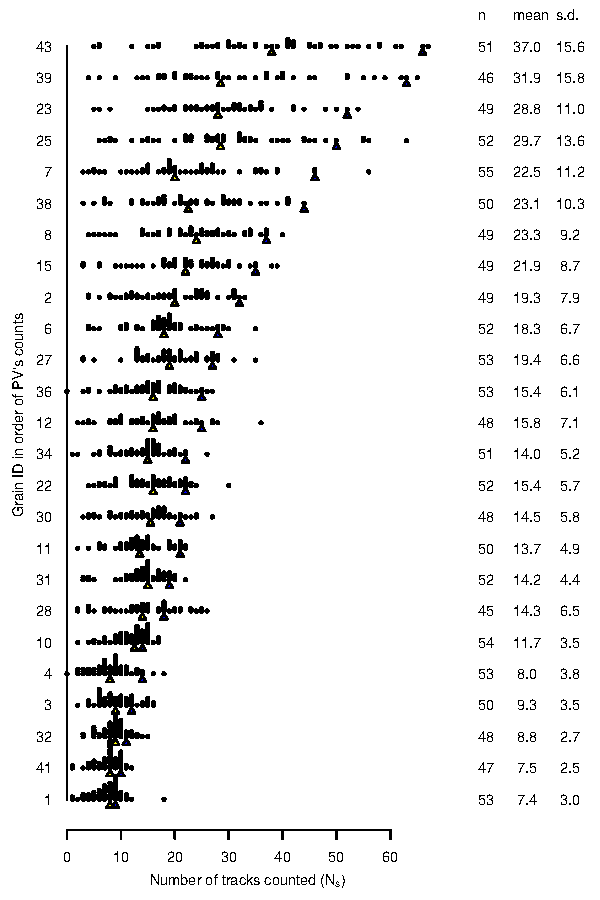
\includegraphics[width=\linewidth]{stripchart.pdf}\medskip
\end{minipage}
\begin{minipage}{.45\linewidth}
\captionof{figure}{Strip chart of the data shown in
  Table~\ref{tab:crowdtable}, with the students' medians and PV's
  counts shown as yellow and blue triangles, respectively.
  \medskip}
  \label{fig:stripchart}
\end{minipage}

As mentioned in Section~\ref{sec:architecture}, geochron@home stores
the actual track positions marked by the users. This raw data can be
downloaded as a \texttt{.json} file and inspected in detail.
Figure~\ref{fig:23vs25}b shows two-dimensional histograms for the x-y
positions of all the track positions generated by the students in
grains~23 and 25. Visual comparison of the histograms with the optical
images confirms that the students unanimously identified the most
obvious semitracks, which contain a clearly visible etch pit and
tail. Shorter and fainter tracks received fewer clicks. Datasets like
this can be used to replace integer counts of fission tracks with
probabilities, reflecting the ambiguity of some fission track
datasets. Figure~\ref{fig:23vs25} also shows that some students
counted the tails of the fission tracks rather than their etch pits,
despite being told the opposite in the tutorial. Fixing this issue
will require some improvements to the tutorial pages
(Section~\ref{sec:outlook}).\medskip

%\begin{figure}[!ht]
{ \centering 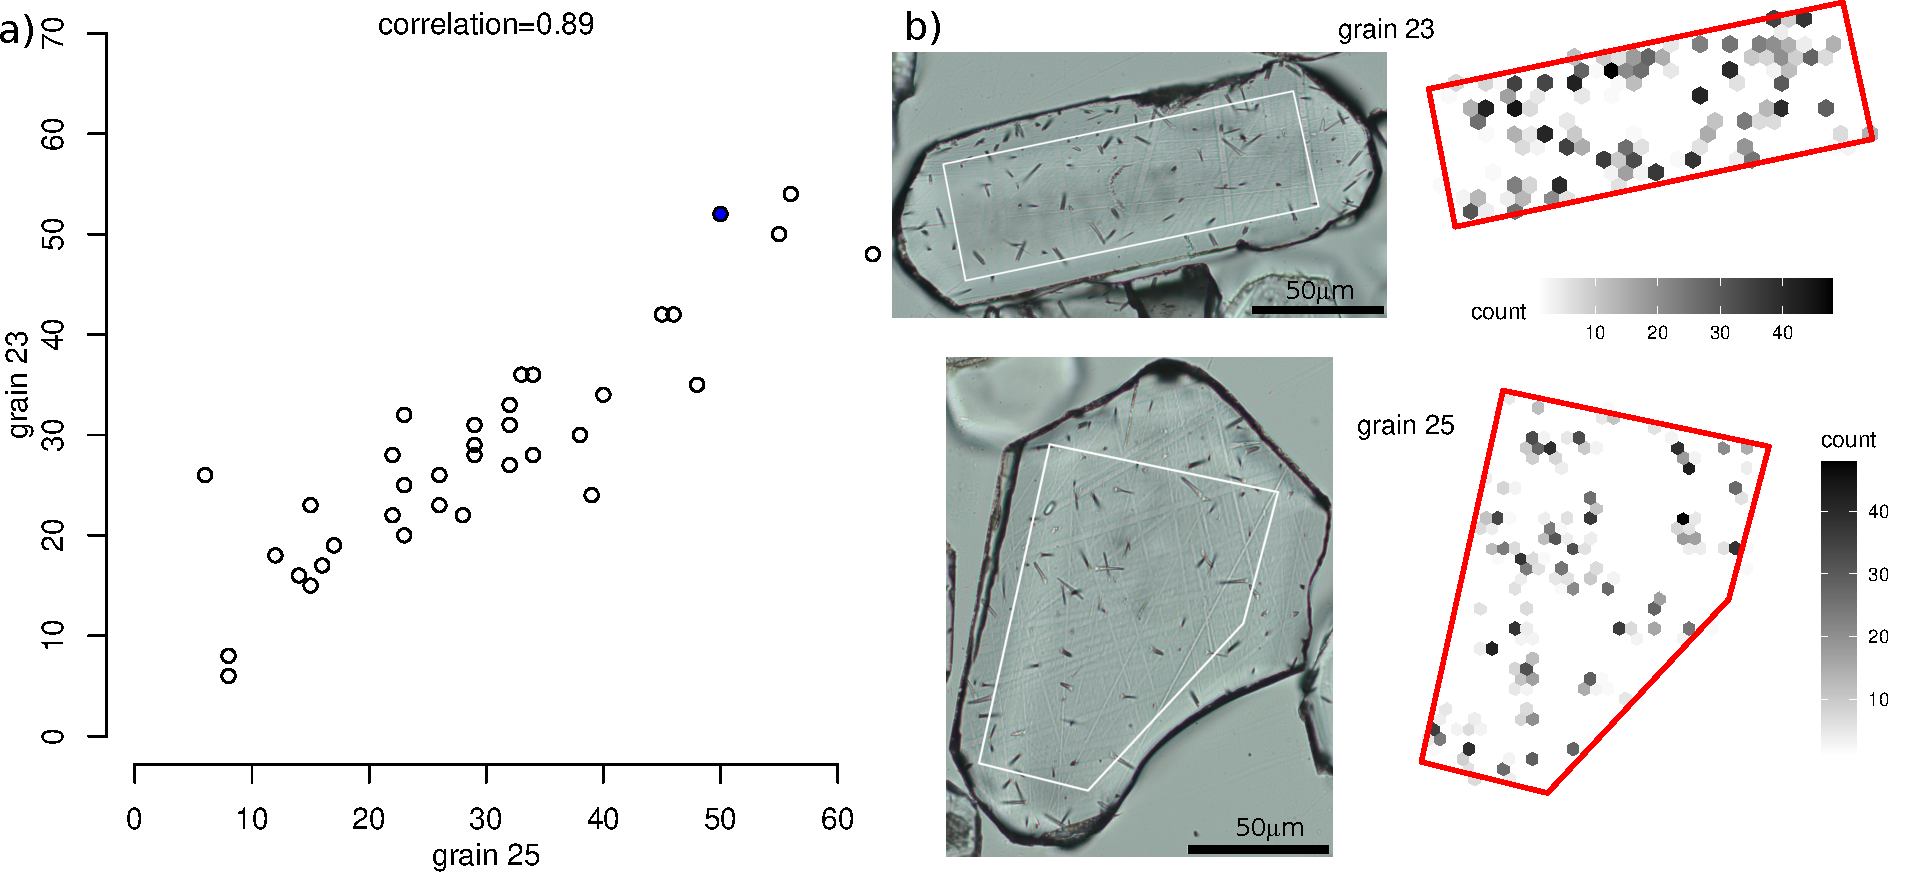
\includegraphics[width=15cm]{23vs25.pdf}
  \captionof{figure}{a) The track counts for grain~23 plotted against
    those for grain 25 for 36 students who counted both of those
    grains. The grey line through the origin has slope 0.97, equal to
    the ratio of the students' total counts for each grain.  The blue
    dot shows PV's counts for those two grains. b) Optical images in
    transmitted light of Mount Dromedary apatites 23 and 25 in the
    crowd-sourcing experiment, along with two-dimensional histogram of
    the track locations for the two grains, as identified by the
    citizen scientists.
    \medskip}
  \label{fig:23vs25}
}%\end{figure}

\section{Outlook}\label{sec:outlook}

geochron@home has been in development for a decade and remains a work
in progress. Planned improvements include:

\begin{enumerate}
\item Length measurements. The geochron@home archive already
  contains horizontally confined fission track measurements
  \citep{tamer2025}.  However, these results must be generated
  externally (e.g., using Fission Track Studio) and uploaded via a
  \texttt{.json} file.  The virtual microscope curently lacks the
  functionality to generate length data within
  geochron@home. This functionality will be added in a future
  update.
\item Dpar and Dper. Etch pits are currently stored as simple sets of
  x- and y-coordinates.  In reality, etch pits have a finite length
  (`Dpar') and width (`Dper'), which serve as useful indicators for
  the horizontal etch rates along the c-axis and parallel to it
  \citep{donelick1993}. Functions will be added to measure and
  visualise this type of data in geochron@home.
\item Interactive tutorial pages and embedded quality
  control. Section~\ref{sec:crowdsourcing} shows that the
  crowd-sourcing idea is not yet ready for general use. Two
  improvements will be made to make its results more reliable. First,
  a `quiz' will be added to the tutorial pages to ensure that novice
  users do not count the tails but the etch pits of fission
  tracks. Only users who click on the `correct' features in an
  unlabelled set of images will be allowed to count new
  samples. Second, future citizen scientists will occasionally be
  served reference images of known track density. Their counts for
  these `test' images will be used to identify trustworthy analysts
  (top of Table~\ref{tab:crowdtable}) and flag unreliable ones (bottom
  of Table~\ref{tab:crowdtable}).
\item Machine learning. Data science is experiencing an artificial
  intelligence (AI) revolution that has already started to transform
  the fission track method \citep{nachtergaele2020}.  Convolutional
  neural networks must be trained with example data. geochron@home is
  ideally suited for this task. Section~\ref{sec:crowdsourcing} showed
  how the opinion of multiple fission track analysts can be combined
  to label fission track images with probabilities rather than
  counts. This data format is close to the form in which data are
  treated within an AI algorithm.
\item Inverse counting. Once trained on historical data, AI algorithms
  can be used to count fission tracks automatically. Following the
  model of Fission Track Studio \citep{gleadow2009, gleadow2019},
  machine learning can be used to reverse the fission track counting
  process. Instead of asking users to count the fission tracks in a
  sample, the software can ask them to check the results proposed by
  an AI algorithm, and to remove any features that are \emph{not}
  fission tracks.  Regardless of whether fission tracks were counted
  manually or with a machine, the value of the geochron@home archive
  remains the same. It is important to document data so that samples
  can be reanalysed in the future, for example when a new and improved
  generation of machine learning algorithms becomes available.
\end{enumerate}

These improvements will be made by ourselves pending additional
funding. However, because geochron@home is free and open software, we
invite any interested parties to join the effort and extend or improve
our code.

\section{Conclusions}\label{sec:conclusions}

This paper introduced geochron@home, a software platform for FAIR
fission track analysis. We demonstrated four different applications of
this platform using real data. Putting the FAIR data paradigm into
practice, all the imagery, counts and source code for this paper are
publicly available on the geochron@home archive. Using these
resources, the reader can reproduce all the results that were
presented in this publication.  We encourage other geochronologists to
follow this example.  FAIR workflows promise to address the
reproducibility crisis in science \citep{miyakawa2020}.\medskip

geochron@home's rich archive of raw data can be reanalysed in
the future. We anticipate that the adoption of FAIR data processing
workflows will open up new research opportunities. For example,
archived pairs of peer-reviewed fission track images and counts could
be used to train the next generation of automated machine learning
algorithms. Conversely, it is also possible that future improvements
in fission track images analysis will be used to update the count data
for published datasets, improving their accuracy.\medskip

Another advantage of the geochron@home workflow is the separation of
image acquisition and image analysis. This separation reduces the
hardware requirements for fission track geochronology. It opens up the
possibility to share resources. State-of-the-art digital microscopes
are expensive. Using geochron@home, a single microscope can serve
multiple users and make fission track analysis more
affordable.\medskip

The fission track method has always been a test bed for new
geochronological developments.  Because fission track data are
imprecise, the fission track community has solicited the help of
statisticians and mathematicians to develop its analytical protocols.
Other geochronological communities are still catching up with concepts
and tools such as overdispersion, mixture modelling and radial plots,
which have been commonplace in fission track analysis for decades
\citep{vermeesch2019b}. In a similar vein, the subjective nature of
fission track identification has prompted the fission track community
to organise inter-laboratory comparisons and round-robin studies long
before other geochronological communities
\citep{miller1985,tamer2025}.\medskip

With the development of geochron@home, fission track thermochronology
is once again ahead of the pack in terms of FAIR data analysis.
geochron@home currently only stores images and counts. This is enough
to reproduce the results of fission track studies using the external
detector method, but not for LA-ICP-MS based data. FAIR data
processing of LA-ICP-MS data requires a new generation of mass
spectrometer data reduction software. We are currently working on this
\citep{vermeesch2025b}. The development of FAIR ICP-MS data pipelines
will not only benefit fission track analysis but other chronometers as
well, such as in-situ U--Pb, Rb--Sr and Lu--Hf.\medskip

With the establishment of FAIR data, geochronology will be well placed
to avoid the reproducibility problems that have plagued other fields
of science.

\codedataavailability{geochron@home is free software released under
  the GPL-3 license. The package and its source code are available
  from \url{https://github.com/pvermees/geochron-at-home} (last
  access: August~21, 2025).  The raw data (imagery) are available at
  the geochron@home archive (\url{https://github.com/pvermees/GaHa},
  last access: August~21, 2025).  R-scripts to reproduce the figures
  are provided in the supplementary information
  (\url{https://github.com/pvermees/supplements}, last access:
  August~21, 2025).}

%\noappendix

\authorcontribution{PV designed the study, acquired the funding and
  counted fission tracks. JH created geochron@home. TB expanded
  geochron@home and wrote the accompanying microscope image
  acquisition software. RG derived Equation~\ref{eq:NO}, designed
  Table~\ref{tab:crowdtable} and verified the other calculations. AC
  provided the samples, prepared the training data and counted fission
  tracks. PV and RG wrote the paper with input from the other
  authors.}

\competinginterests{PV is an Associate Editor of \emph{Geochronology}.}

\begin{acknowledgements}
This research has been supported by the Natural Environment Research
Council (grant no. NE/T001518/1), awarded to Pieter Vermeesch. We would like
to thank the students of GEOL0017 (`Isotope Geology') for their contribution
to the crowd-sourcing experiment of Section~\ref{sec:crowdsourcing}.
\end{acknowledgements}

\bibliographystyle{copernicus}
\bibliography{biblio.bib}

\end{document}
